\chapter{计数与计算}
\label{chap:combinatorics}

第~\ref{chap:sets-functions-and-proofs}章已建立集合、函数、索引族与逻辑陈述的语言。
现在考察离散对象的结果空间，以及对这些对象提出的求解任务。
同样一组候选，可以问有多少种不同结果、哪些结果满足规则、哪一个目标值最好；还可以
问是否存在处理所有合法输入的统一程序，以及程序需要多少资源。这些问题相互关联，
但结果数量不能直接给出必需的枚举成本，模式容量也不能代替算法复杂度。

本章用二值选择说明它们的分工。对非负整数$n$，令
\[
  V=\{1,\ldots,n\},\qquad
  \bm z=(z_i)_{i\in V}\in\{0,1\}^n,\qquad
  S(\bm z)=\{i\in V:z_i=1\}.
\]
赋值与子集是同一选择的两种表示。在贯穿例子中记$V_0=\{1,2,3,4\}$，
回用前章式~\eqref{eq:comb-running-cnf}的四候选规则：
候选$1$与$2$恰选一个，候选$3$依赖$1$，候选$4$要求$2$或$3$至少出现一个。
集合计数研究这些表示的数量和贡献结构；函数族限制到有限输入后，则得到可计数的标记模式。
规则与目标随后定义判定、搜索和优化任务，程序理论再对整类输入讨论可计算能力与资源。
最后一种考察不限于这个小例子，也不限于有限候选的枚举。

\section{候选空间的结构与计数}
\label{sec:comb-families-counting}

数量比较必须固定结果对象：一个有序选择、一个子集和一个输入上的标记模式，不能混用
同一种计数口径。以下先建立精确计数及增长尺度，再分别处理重叠校正、局部贡献恢复和
函数族的模式容量；这些结论刻画结果空间，不预先断言求解程序必须怎样运行。

\subsection{集合族与候选规模}

第~\ref{chap:sets-functions-and-proofs}章已经区分集合、序列和索引族。计数时还要
确定哪些表示属于同一个结果，再研究规则改变后候选数量怎样变化。一个\term{集合族}（set family）
$\mathcal{F}\subseteq\mathcal{P}(V)$是一组允许讨论的子集。若不加任何限制，
$\mathcal{F}=\mathcal{P}(V)$；各元素选择与否不受其他元素约束，所以
\begin{equation}
  |\mathcal{P}(V)|=2^n.
  \label{eq:comb-power-set-count}
\end{equation}

候选由若干选择组成时，需要知道共有多少种不同结果。计数时必须先确定，交换选择次序是否得到同一个对象。
设$n,k$为整数且$0\leq k\leq n$。从$n$个不同对象中依次取出$k$个且不放回，
若顺序重要，可得到
\[
  P(n,k)=n(n-1)\cdots(n-k+1)=\frac{n!}{(n-k)!}
\]
种排列。若只关心选中了哪些对象，不关心次序，每个大小为$k$的子集被计算了$k!$次，
因此组合数为
\begin{equation}
  \binom{n}{k}=\frac{n!}{k!(n-k)!},
  \qquad 0\leq k\leq n.
  \label{eq:prelim-binomial-coefficient}
\end{equation}
规定$\binom{n}{k}=0$用于$k<0$或$k>n$，可以统一许多边界公式。

把$n$个对象的子集按是否包含某个固定对象分组，可得Pascal恒等式
\[
  \binom{n}{k}
  =
  \binom{n-1}{k}
  +
  \binom{n-1}{k-1}.
\]
第一项计算不包含固定对象的子集，第二项先包含该对象，再从其余$n-1$个对象中选择
$k-1$个。这种“为同一集合建立不重不漏的两种计数”称为组合证明。下面的容斥与子集反演会继续利用这种有限分组与抵消的思路。

二项式定理把组合数与代数展开连接起来：
\begin{equation}
  (a+b)^n
  =
  \sum_{k=0}^{n}\binom{n}{k}a^k b^{n-k}.
  \label{eq:prelim-binomial-theorem}
\end{equation}
选择展开式中的一项时，需要从$n$个因子中挑出$k$个贡献$a$，其余贡献$b$，所以
$a^k b^{n-k}$前的系数正是$\binom{n}{k}$。概率论中的二项分布和学习理论中的有限类
计数都会复用这个关系。

例如，从$\{1,2,3,4\}$中取两个元素有$12$个有序对，却只有$6$个二元子集；
$(1,3)$与$(3,1)$在前一个任务中不同，在后一个任务中表示同一个结果。

幂集的数量也可按子集大小分层计算，再由二项式定理得到
$\sum_{k=0}^{n}\binom{n}{k}=(1+1)^n=2^n$。二值选择与按大小分层是两种计数口径，
计算的是同一批子集。

每个$S\subseteq V$也确定一个有序二分划分$(S,V\setminus S)$，所以有序二分划分
仍有$2^n$个。若两部分没有名称，$(S,V\setminus S)$与$(V\setminus S,S)$表示
同一个划分；当$n\geq1$时没有子集等于自己的补集，每个无序划分恰被计算两次，数量为
$2^{n-1}$。是否区分两侧决定了计数对象，不能只看它们都把$V$分成两部分。
这里允许某一部分为空；若要求两部分都非空，有序与无序数量应分别减为
$2^n-2$与$2^{n-1}-1$。当$n=0$时，交换两侧不会产生两个不同表示，上述除以$2$的
论证也不适用。

若只允许恰好选择$k$项，集合族变为
\[
  \binom{V}{k}=\{S\subseteq V:|S|=k\},
  \qquad
  \left|\binom{V}{k}\right|=\binom{n}{k}.
\]
若允许至多选择$k$项，则数量为$\sum_{j=0}^{k}\binom{n}{j}$。因此“候选总数有限”
仍可能掩盖完全不同的增长规模：固定$k$时，该和关于$n$至多按$n^k$增长；
$k$随$n$线性增长时，候选数却可能接近$2^n$。

计数常可通过一个变量把问题拆成两个较小问题。记$a_{n,k}$为从$n$个元素中选择
$k$个的方案数。对$n\geq1$，固定元素$n$后，所有方案被不重不漏地分成“不含$n$”
与“含$n$”两类。为使边界项也有定义，约定$a_{0,0}=1$，并在$k<0$或$k>n$时令
$a_{n,k}=0$。于是对$n\geq1$和任意整数$k$都有
\begin{equation}
  a_{n,k}=a_{n-1,k}+a_{n-1,k-1}.
  \label{eq:comb-binomial-recurrence}
\end{equation}
这既是Pascal恒等式，也是一个递推算法。

\subsection{计数与代价的增长尺度}
\label{sec:comb-growth-scales}

候选数量与算法成本都可能随输入规模变化，精确值不同的两个序列也可能具有同一增长尺度。设$a_n$与$b_n$为实数序列，且从某个位置开始
$b_n>0$。若存在常数$C>0$和$n_0$，使得
\[
  \forall n\geq n_0,\qquad |a_n|\leq Cb_n,
\]
则记$a_n=O(b_n)$。这表示$a_n$的绝对值最终被$b_n$的常数倍控制，常数$C$不随$n$
改变。若对任意$\varepsilon>0$，都存在$n_\varepsilon$使
\[
  \forall n\geq n_\varepsilon,\qquad |a_n|\leq\varepsilon b_n,
\]
则记$a_n=o(b_n)$。这要求最终能用任意小的正比例控制$a_n$，比一个固定常数倍的界更强。
第~\ref{chap:mathematical-analysis}章会把它表述为比值趋于零，并用于函数的局部余项。

例如$n=O(n)$、$3n+7=O(n)$且$\log n=o(n)$。但大O不是精确等式：
$n=O(n^2)$也成立，只是界较松。写算法复杂度时还要说明被计数的操作、输入规模和计算
模型；写统计误差时则要说明界是确定性的、期望意义的还是以高概率成立
\scite{math-graham1994concrete}

当序列还依赖维数$d$或其他规模时，也要说明哪些量允许进入隐含常数。例如，对每个固定
$d$都有$d/n=O(1/n)$，因为可以取$C=d$；但若要求同一个$C$同时适用于任意$d$，这个
界就不成立。因此，“关于$n$是某个速率”不等于该速率对维数一致。需要一致结论时，应把
量词写成对所讨论的全部$d$使用同一组$C$与$n_0$，或把$d$显式保留在界中。

对迭代序列，常用$t$而不是$n$表示步数。若目标$F:\mathbb{R}^d\to\mathbb{R}$
有有限下确界，记$F^\star=\inf_{\bm{w}\in\mathbb{R}^d}F(\bm{w})$；达到它的
参照最小点（若存在）记为$\bm{w}^\star$。例如
\[
  F(\bm{w}^{(t)})-F^\star=O(1/t)
\]
表示存在与$t$无关的常数控制目标值误差。这个式子没有说明参数误差
$\lVert\bm{w}^{(t)}-\bm{w}^\star\rVert_2$具有同样速率，也没有说明一次迭代的成本。
比较算法时，必须固定误差对象和成本口径。

前一小节的组合数递推也可以按这个口径评估。
若只保存上一行，计算全部
$a_{n,0},\ldots,a_{n,n}$需要$O(n^2)$次加法和$O(n)$个存储单元。
闭式公式、递推关系和计算过程由此承担不同作用：闭式便于分析规模，递推揭示分组结构，
算法还必须说明求值顺序和资源。

\subsection{容斥原理与重复计数}

直接把若干坏情形的数量相加会重复计算同时违反多条规则的赋值。
\term{容斥原理}（inclusion--exclusion principle）用交集项逐层校正这种重复。

\begin{theorem}[有限容斥原理]
\label{thm:comb-inclusion-exclusion}
设$A_1,\ldots,A_m$是有限集合。则
\begin{equation}
  \left|\bigcup_{i=1}^{m}A_i\right|
  =
  \sum_{\varnothing\neq I\subseteq\{1,\ldots,m\}}
  (-1)^{|I|+1}
  \left|\bigcap_{i\in I}A_i\right|.
  \label{eq:comb-inclusion-exclusion}
\end{equation}
\end{theorem}

\begin{proof}
固定任意元素$x$，设它恰好属于$r$个集合。若$r=0$，它在等式两侧都没有贡献。
若$r\geq1$，右侧从含有$x$的$r$个集合中选择非空索引集，给$x$计算的总系数为
\[
  \sum_{k=1}^{r}(-1)^{k+1}\binom{r}{k}
  =
  1-\sum_{k=0}^{r}(-1)^k\binom{r}{k}
  =1-(1-1)^r=1.
\]
所以并集中的每个元素在右侧恰好被计算一次，对所有$x$求和即得结论。
\end{proof}

回到$V_0$上的四个变量。把三条规则的违反事件记为
\[
  \begin{aligned}
    A_1&=\{\bm{z}:z_1=z_2\},\\
    A_2&=\{\bm{z}:z_3=1,\ z_1=0\},\\
    A_3&=\{\bm{z}:z_4=1,\ z_2=0,\ z_3=0\}.
  \end{aligned}
\]
它们分别表示基础标签没有恰选一个、缺少候选$1$时仍选择候选$3$，以及候选$4$缺少前提。
全部赋值有$16$个，并且
\[
  |A_1|=8,\quad |A_2|=4,\quad |A_3|=2.
\]
交集大小为
\[
  |A_1\cap A_2|=2,\qquad
  |A_1\cap A_3|=1,\qquad
  |A_2\cap A_3|=|A_1\cap A_2\cap A_3|=0.
\]
由式~\eqref{eq:comb-inclusion-exclusion}，坏赋值共有
$8+4+2-2-1=11$个，因此可行赋值有$16-11=5$个。它们对应
\begin{equation}
  \mathcal{C}_0
  =
  \bigl\{
  \{1\},\{1,3\},\{1,3,4\},\{2\},\{2,4\}
  \bigr\}.
  \label{eq:comb-running-feasible-family}
\end{equation}
这些集合恰是前章式~\eqref{eq:comb-running-cnf}的全部模型。
第~\ref{sec:comb-logic-constraints}节将区分检查、判定与搜索对这批对象所要求的回答。

\subsection{子集格上的 Möbius 反演}

容斥处理的是若干集合的重叠。一个更一般的问题是：若已知每个$S$上的总量由其全部
子集贡献累加而成，能否还原每个子集自身新增的贡献？子集按包含关系形成前章定义的偏序。两个子集的交是包含于两者的最大子集，
并则是包含两者的最小子集；这种带有交、并运算的子集偏序称为子集格。
\term{Möbius反演}（Möbius inversion）给出这一累加变换的逆。

\begin{theorem}[子集格上的 Möbius 反演]
\label{thm:comb-mobius-inversion}
设$g,h:\mathcal{P}(V)\to\mathbb{R}$满足
\begin{equation}
  g(S)=\sum_{T\subseteq S}h(T)
  \qquad\text{对每个 }S\subseteq V.
  \label{eq:comb-zeta-transform}
\end{equation}
则
\begin{equation}
  h(S)
  =
  \sum_{T\subseteq S}(-1)^{|S|-|T|}g(T).
  \label{eq:comb-mobius-inversion}
\end{equation}
反过来，由式~\eqref{eq:comb-mobius-inversion}定义$h$也会恢复
式~\eqref{eq:comb-zeta-transform}。
\end{theorem}

更一般的有限偏序集把$T\subseteq S$换成$T\preceq S$。其Möbius函数由
$\mu(S,S)=1$以及
$\mu(T,S)=-\sum_{T\preceq R\prec S}\mu(T,R)$（$T\prec S$）递归确定，
不满足$T\preceq S$时取$\mu(T,S)=0$。反演系数不再只由
$|S|-|T|$决定。本章只使用子集格，此时递归解恰为
$\mu(T,S)=(-1)^{|S|-|T|}$。

\begin{proof}
把式~\eqref{eq:comb-zeta-transform}代入反演式右侧并交换有限求和次序，得到
\begin{align*}
  \sum_{T\subseteq S}(-1)^{|S|-|T|}g(T)
  &=
  \sum_{T\subseteq S}(-1)^{|S|-|T|}
  \sum_{R\subseteq T}h(R)\\
  &=
  \sum_{R\subseteq S}h(R)
  \sum_{T:R\subseteq T\subseteq S}
  (-1)^{|S|-|T|}.
\end{align*}
固定$R$后，中间集合$T$由$S\setminus R$中哪些元素被加入决定。若
$q=|S\setminus R|$，内层和等于
\[
  \sum_{j=0}^{q}\binom{q}{j}(-1)^{q-j}
  =(1-1)^q.
\]
它在$R=S$时为$1$，在$R\neq S$时为$0$，所以全部较小子集的贡献抵消，只留下
$h(S)$。同一抵消关系也证明反向代入恢复$g$。
\end{proof}

在小集合$V_0$上，假设累计得分具有形式
\[
  g(S)
  =
  2|S|
  +3\mathbb{I}\{\{1,3\}\subseteq S\}
  -\mathbb{I}\{\{2,4\}\subseteq S\}.
\]
每个单项贡献$2$，组合$\{1,3\}$额外贡献$3$，而组合$\{2,4\}$产生$-1$的交互。
四个元素共有$16$个子集。把每个子集的累计值与反演恢复的局部贡献并列，可以完整核对
正向累加与反向消去：
\begin{table}[htbp]
  \centering
  \caption{四元素子集格上的累计值与局部贡献。除四个单项、交互
  $\{1,3\}$和$\{2,4\}$外，其余局部贡献均为零。}
  \label{tab:comb-four-element-mobius}
  \begin{tabular}{ccc@{\qquad}ccc}
    \toprule
    $S$ & $g(S)$ & $h(S)$ & $S$ & $g(S)$ & $h(S)$ \\
    \midrule
    $\varnothing$ & $0$ & $0$ & $\{1,2\}$ & $4$ & $0$ \\
    $\{1\}$ & $2$ & $2$ & $\{1,3\}$ & $7$ & $3$ \\
    $\{2\}$ & $2$ & $2$ & $\{1,4\}$ & $4$ & $0$ \\
    $\{3\}$ & $2$ & $2$ & $\{2,3\}$ & $4$ & $0$ \\
    $\{4\}$ & $2$ & $2$ & $\{2,4\}$ & $3$ & $-1$ \\
    $\{3,4\}$ & $4$ & $0$ & $\{1,2,3\}$ & $9$ & $0$ \\
    $\{1,2,4\}$ & $5$ & $0$ & $\{1,3,4\}$ & $9$ & $0$ \\
    $\{2,3,4\}$ & $5$ & $0$ & $V_0$ & $10$ & $0$ \\
    \bottomrule
  \end{tabular}
\end{table}
若只观察各子集的累计值，反演给出
\[
  h(\{i\})=g(\{i\})-g(\varnothing)=2,
\]
以及
\[
  \begin{aligned}
  h(\{1,3\})
  &=g(\{1,3\})-g(\{1\})-g(\{3\})+g(\varnothing)=3,\\
  h(\{2,4\})
  &=g(\{2,4\})-g(\{2\})-g(\{4\})+g(\varnothing)=-1.
  \end{aligned}
\]
其余大小至少为$2$的局部贡献均为零。反演并没有假设贡献为正；它只保证累计量与局部
交互之间可以互相重构。

例如对$S=\{1,2,3\}$，累计值为$g(S)=9$，三个二元子集的累计值依次为
$4,7,4$，三个单元素累计值之和为$6$，且$g(\varnothing)=0$。反演确实给出
\[
  h(\{1,2,3\})=9-(4+7+4)+6-0=0.
\]
把已经恢复的单项贡献$2,2,2$与二元贡献$3$重新相加，也得到
$g(\{1,2,3\})=9$。正向累加与反向消去由此可以在同一组数值上相互复核。

图~\ref{fig:comb-mobius-cumulative-local}只保留$\{1,3\}$的四个子集，比较累计量与局部量。
累计值$g(\{1,3\})=7$包括两个单项的$2$以及共同出现才增加的$3$；反演消去两个单项后，
留下的是交互贡献$3$，并不是把累计值本身改成负数或丢掉较小子集。
\begin{figure}[htbp]
 \centering
 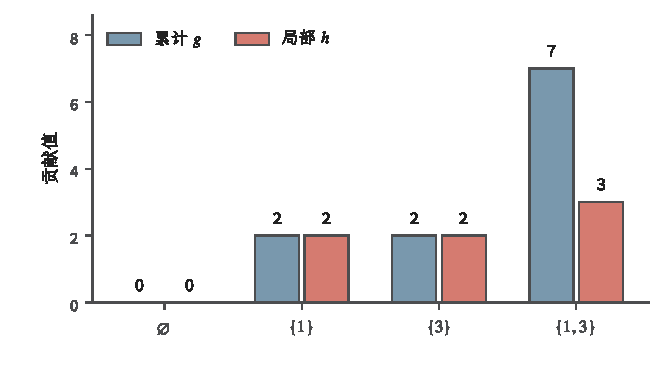
\includegraphics[width=\linewidth]{figures/math-preparation/reader-revision-analysis/combinatorics-mobius-cumulative-local.pdf}
 \caption{同一四元素教学构造在$\{1,3\}$的子集上的累计值与局部贡献。蓝柱为$g$，红柱为$h$；
 单项贡献各为$2$，二元累计值$7$包含额外交互$3$。图中四个子集的数据由正文解析式精确计算，
 没有省略影响这个二元交互的子集。}
 \label{fig:comb-mobius-cumulative-local}
\end{figure}

容斥原理可以看成同一反演机制作用于指示函数。正负号
$(-1)^{|S|-|T|}$不是需要另行记忆的巧合，而是“所有严格更小子集相互抵消”所需的系数。
后续图模型会把这一重构用于变量子集间的局部交互，再用图结构限制哪些交互允许出现。
Möbius反演本身只是一条有限集合恒等式，不会自动给出这些结构限制，也不保证所得局部项非负。

\subsection{二值函数族的标记模式与容量}
\label{sec:comb-label-family-capacity}

集合族的计数固定了已给出的候选规则。函数类的比较还要允许输入点改变，
并控制任意有限输入组上能实现多少种输出模式。把标记向量看作集合后，
同样的递推计数可建立VC维与多类别维度的界；实值输出则用阈值与间隔区分数值选择。
这里研究的是模式丰富度，
统计误差还需概率条件，求解代价还需程序与编码；模式容量本身不能回答这两类问题。

\subsubsection{限制类与可实现标记}

无限函数类在有限输入上只留下有限个二值标记。这里把每种标记改写成一个子集，再用能够实现多少种模式来刻画它的组合丰富度；第~\ref{chap:probability-theory}章则把这种有限化用于同时误差控制。
给定输入$x_1,\ldots,x_m$和二值函数类$\mathcal{H}$，每个$h\in\mathcal{H}$确定
\[
  A_h=\{i\in\{1,\ldots,m\}:h(x_i)=1\}.
\]
函数在这组输入上的标记向量与$A_h$一一对应，因此不同标记的数量就是集合族
$\{A_h:h\in\mathcal{H}\}\subseteq\mathcal{P}(\{1,\ldots,m\})$的大小。式~
\eqref{eq:comb-power-set-count}随即给出上界$2^m$；生长函数只是在所有输入组中取这个
数量的上确界。

下列定义针对非空输入空间上的非空二值函数类
\(\mathcal H\subseteq\{0,1\}^{\mathcal X}\)，不涉及抽样分布。
把输入集\(C=\{x_1,\ldots,x_m\}\)按所列次序排列，在\(C\)上的限制类
记录这组输入上全部可实现的标记向量：
\[
  \mathcal H|_C=\{(h(x_1),\ldots,h(x_m)):h\in\mathcal H\}.
\]
\begin{definition}[打散]
  \label{def:shattering}
  若对有限互异输入集\(C\)的每个二值标记\((b_1,\ldots,b_m)\)，都存在\(h\in\mathcal H\)满足\(h(x_i)=b_i\)对全部\(i\)成立，就称\(\mathcal H\)\term{打散}（shatter）\(C\)。等价地，\(\mathcal H|_C=\{0,1\}^m\)。
\end{definition}
\begin{definition}[VC维]
  \label{def:vc-dimension}
  \(\mathcal H\)的\term{VC维}（Vapnik--Chervonenkis dimension）为
  \[
    \operatorname{VC}(\mathcal H)
    =\sup\{|C|:C\subseteq\mathcal X,\ |C|<\infty,\ C\text{被}\mathcal H\text{打散}\}.
  \]
  空集总能被非空函数类打散，所以维度可为\(0\)；若任意大有限集都能被打散，则取值为\(+\infty\)。
\end{definition}
\begin{definition}[生长函数]
  \label{def:growth-function}
  对整数\(m\geq0\)，定义
  \begin{equation}
    \Pi_{\mathcal H}(m)
    =\max_{x_1,\ldots,x_m\in\mathcal X}
    |\{(h(x_1),\ldots,h(x_m)):h\in\mathcal H\}|.
    \label{eq:growth-function}
  \end{equation}
  \(m=0\)时只有一个空标记，故\(\Pi_{\mathcal H}(0)=1\)。
\end{definition}
VC维记录可完整实现全部模式的最大输入集大小；生长函数记录任意给定输入数下最多实现多少模式。输入可重复的约定使有限输入空间上的式~\eqref{eq:growth-function}也对全部\(m\)有定义；重复输入不会产生新的独立标记位。

这个表示还能直接计算受基数约束的函数族。令$\mathcal{X}$为无限集，固定$k\geq0$，并设
\[
  \mathcal{H}_k
  =
  \{h_S:S\subseteq\mathcal{X},\ |S|\leq k\},
  \qquad
  h_S(x)=\mathbb{I}\{x\in S\}.
\]
对$m$个互异输入，$\mathcal{H}_k$能够实现的正类索引集合恰是所有大小不超过$k$的
子集，因而
\[
  \Pi_{\mathcal{H}_k}(m)
  =
  \sum_{j=0}^{\min\{k,m\}}\binom{m}{j}.
\]
固定$k$时，这个数量关于$m$至多按$m^k$增长；当$k\geq m$时，它恢复为$2^m$。
同一个幂集计数由此区分出多项式规模与指数规模。它仍只描述有限输入上的模式数，
不直接给出统计误差界，也不保证能够高效找到实现某种标记的函数。

一个可逐项复核的例子是实数轴上的区间分类器。令
$x_1<\cdots<x_m$互异，函数$h_{a,b}(x)=\mathbb{I}\{a\leq x\leq b\}$把落在某个
闭区间内的输入标为$1$。非空正类索引必为连续块
$\{i,i+1,\ldots,j\}$，这样的块由$1\leq i\leq j\leq m$唯一确定；再加上空正类，
可实现模式数恰为
\[
  1+\sum_{i=1}^{m}(m-i+1)
  =
  1+\frac{m(m+1)}2.
\]
当$m=3$时，七个模式为$000,100,010,001,110,011,111$，只有$101$无法实现。
因此三个有序点不能被该函数类打散；两个点的四种模式都能实现。这个算例也说明，
参数$a,b$取值无限多，并不意味着有限输入上的标记模式也有无限多个。

图~\ref{fig:comb-interval-shattering-patterns}把“每一种模式”逐项展开。两个点的四种标记
都能由一个区间实现；三个点的$101$要求包含两端却排除中点，违背区间的连续块结构。
图~\ref{fig:combinatorics-growth-patterns}随后只保留模式数量，两张图分别回答实现结构与增长规模。
\begin{figure}[htbp]
 \centering
 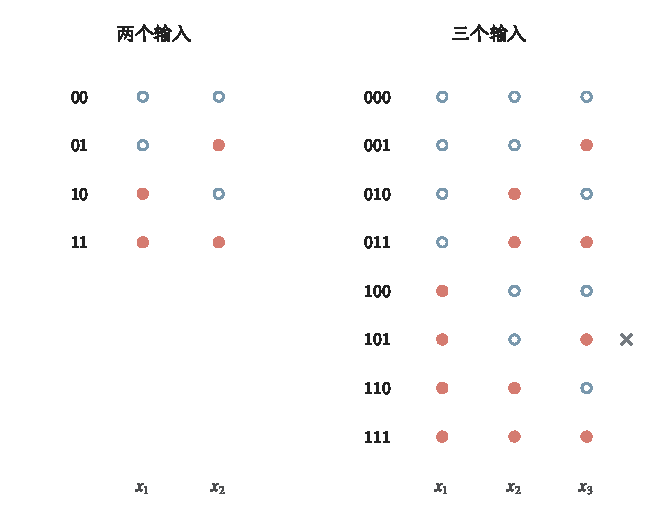
\includegraphics[width=\linewidth]{figures/math-preparation/reader-revision-analysis/combinatorics-interval-shattering-patterns.pdf}
 \caption{区间分类器在互异有序输入上的全部二值模式。红实心点表示标记$1$，蓝空心点表示标记$0$；
 每行是一种模式。左侧两个输入的四行全部可实现，右侧三个输入仅$101$不可实现，灰色叉号标出缺失行。
 这是精确的有限模式构造，不是抽样统计。}
 \label{fig:comb-interval-shattering-patterns}
\end{figure}

图~\ref{fig:combinatorics-growth-patterns}把区间类与全部标记放在对数轴上比较。区间类的两个端点参数虽有无穷多种取值，有限输入上的模式数却仅按平方增长。计数相同也不表示函数类相同：当\(k=2\)时，\(\mathcal H_k\)的模式数同样为\(1+m(m+1)/2\)，但在三个点上它缺少\(111\)，区间类却缺少\(101\)。因此生长函数约束丰富程度，并不完整记录模式的结构。

\begin{figure}[htbp]
  \centering
  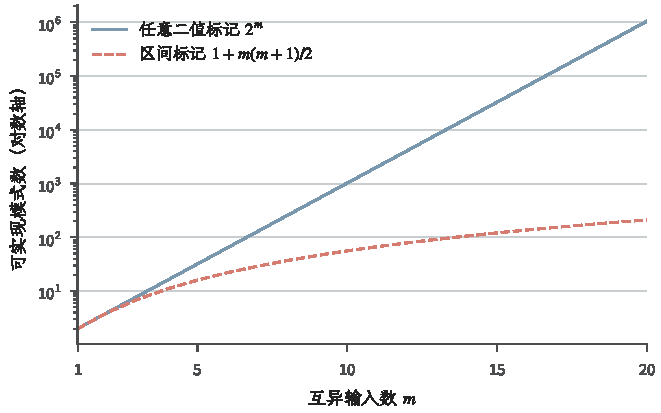
\includegraphics[width=\linewidth]{figures/math-preparation/probability-discrete/combinatorics-growth-patterns.pdf}
  \caption{有限输入上的二值模式数（精确计数教学图）。蓝实线为不受限制的\(2^m\)，红虚线为实数轴区间分类器的\(1+m(m+1)/2\)。纵轴使用对数刻度，红线是该具体类的精确计数；它也恰等于至多两个正类点的集合族计数，但两类实现的模式可以不同。}
  \label{fig:combinatorics-growth-patterns}
\end{figure}

\subsubsection{VC维与Sauer--Shelah计数界}
\label{sec:comb-vc-growth}

区间例子的VC维为\(2\)，而模式数恰好达到\(1+m+\binom m2\)。下面的计数界解释为何有限VC维足以限制全部输入上的增长，证明复用式~\eqref{eq:comb-binomial-recurrence}的“最后一个坐标”分组，但需要同时记录哪些旧模式能够接上两个不同标签。
\begin{lemma}[Sauer--Shelah引理]
  \label{lem:sauer-shelah}
  若\(d=\operatorname{VC}(\mathcal H)<\infty\)，则对任意\(m\geq0\)，
  \[
    \Pi_{\mathcal H}(m)\leq\sum_{j=0}^{\min\{d,m\}}\binom mj.
  \]
  特别地，当\(1\leq d\leq m\)时，
  \begin{equation}
    \Pi_{\mathcal H}(m)\leq\sum_{j=0}^{d}\binom mj
    \leq\left(\frac{em}{d}\right)^d.
    \label{eq:sauer-shelah}
  \end{equation}
\end{lemma}
\begin{proof}
固定\(m\)个输入上的有限模式族\(\mathcal A\subseteq\{0,1\}^m\)。令\(U\)为删去末坐标后的所有模式，\(V\subseteq U\)为既能接\(0\)又能接\(1\)的模式，则
\( |\mathcal A|=|U|+|V|\)。\(U\)不能打散超过\(d\)个坐标。\(V\)也不能打散\(d\)个坐标，否则在这些坐标上任意赋值，再把末坐标任意取\(0\)或\(1\)，就会由\(\mathcal A\)打散\(d+1\)个坐标，产生矛盾。

对坐标数归纳。零坐标时至多一个模式；\(d=0\)时也至多一个模式，因为两个不同模式在某一坐标取值不同，便会打散一个坐标。对\(m,d\geq1\)，归纳假设和上面的分组给出
\[
  |\mathcal A|
  \leq\sum_{j=0}^{d}\binom{m-1}{j}
       +\sum_{j=0}^{d-1}\binom{m-1}{j}
  =\sum_{j=0}^{d}\binom mj,
\]
其中超过坐标数的组合数约定为零。重复输入不会增大模式数，因此对全部输入组取最大值得到第一项结论。

当\(1\leq d\leq m\)时，令\(a=d/m\in(0,1]\)。对\(j\leq d\)有\(a^d\leq a^j\)，故
\[
  a^d\sum_{j=0}^{d}\binom mj
  \leq\sum_{j=0}^{d}\binom mj a^j
  \leq(1+a)^m\leq e^{am}=e^d.
\]
除以\(a^d\)便得到简化界。\(d=0\)时第一项界为\(1\)，不使用含\(d\)作分母的简化式。
\end{proof}
引理只给出计数，不直接给出概率保证，也不保证能高效找到实现某种标记的函数。固定\(d\)后，计数上界至多按\(m^d\)增长；具体类可以更慢。要控制经验平均，还需第~\ref{chap:probability-theory}章中的抽样、可测性和集中条件。

\subsection{多类别标记族的组合维度}
\label{sec:comb-multiclass-dimensions}

两个标签时，每个点只有一种与当前标签不同的选择；三个以上标签时，“改为另一个标签”却不唯一。例如两个输入上的六个模式
\[
  \mathcal V=\{(a,a),(a,b),(b,b),(b,c),(c,c),(c,a)\}
\]
没有包含任何固定两标签对的四角矩形，但每个模式都能只改变任一坐标而仍留在\(\mathcal V\)中。完整二元立方体与局部逐坐标歧义不再是同一条件，需要把所允许的标签选择写进定义。

图~\ref{fig:comb-multiclass-pattern-grid}把这个有限例子放进两坐标表格。沿一行移动
只改变第二个标签，沿一列移动只改变第一个标签；每个实心点都能沿两种方向找到另一个
实心点，但没有任取两行两列形成的四个角同时占满。局部可改变与完整二选一组合由此
可以直接区分。
\begin{figure}[htbp]
 \centering
 \figurefont\footnotesize\color{FigureInk}
 \renewcommand{\arraystretch}{1.6}
 \begin{tabular}{cccc}
 \toprule
 第一坐标$\backslash$第二坐标 & $a$ & $b$ & $c$\\
 \midrule
 $a$ & $\bullet$ & $\bullet$ & $\circ$\\
 $b$ & $\circ$ & $\bullet$ & $\bullet$\\
 $c$ & $\bullet$ & $\circ$ & $\bullet$\\
 \bottomrule
 \end{tabular}
 \caption{六模式族$\mathcal V$的精确占位图。实心点表示模式属于该族，空心点表示缺失模式。每行每列恰有两个实心点，却没有完整的四角矩形；这不是两个标签的完整立方体。}
 \label{fig:comb-multiclass-pattern-grid}
\end{figure}

本小节设\(\mathcal H\subseteq Y^X\)非空，\(X,Y\)为非空集合。有限点集中的输入均互异，\(\mathcal H|_C\)依固定的输入次序写成标记向量。以下维度均取可打散有限集大小的上确界，允许\(0\)与\(+\infty\)。

\begin{definition}[Natarajan打散与Natarajan维]
\label{def:natarajan-dimension}
设$C=\{x_1,\ldots,x_m\}\subseteq X$。若存在$f,g:C\to Y$，满足
$f(x)\neq g(x)$对所有$x\in C$成立，且对每个$B\subseteq C$都存在$h_B\in\mathcal H$使
\begin{equation}
 h_B(x)=\begin{cases}f(x),&x\in B,\\g(x),&x\in C\setminus B,\end{cases}
 \label{eq:natarajan-shattering}
\end{equation}
则称$C$被$\mathcal H$ \term{Natarajan打散}（Natarajan shattering）。令$\mathcal C_N$为所有被
$\mathcal H$ Natarajan打散的有限输入集组成的集合，定义
\[
 d_N(\mathcal H)=\sup_{C\in\mathcal C_N}|C|.
\]
\end{definition}

\begin{definition}[图打散]
\label{def:graph-dimension}
若有限集$C\subseteq X$存在$f:C\to Y$，使每个$B\subseteq C$都对应某个
$h_B\in\mathcal H$，满足
\[
 h_B(x)=f(x)\ (x\in B),\qquad h_B(x)\neq f(x)\ (x\in C\setminus B),
\]
则称$C$被$\mathcal H$图打散。
\end{definition}

\begin{definition}[图维]
\label{def:graph-dimension-value}
设$\mathcal C_G$为所有被$\mathcal H$图打散的有限输入集组成的集合，定义
\[
 d_G(\mathcal H)=\sup_{C\in\mathcal C_G}|C|.
\]
\end{definition}

Natarajan打散固定了每个输入上的两个候选标签，图打散只固定一个基准标签；偏离基准时具体采用哪个标签可以随子集改变。为了描述前面六模式例子中的局部邻接，还需一个不预先固定标签对的对象。

\begin{definition}[伪立方体]
\label{def:pseudocube}
有限非空集合$V\subseteq Y^m$称为$m$维伪立方体，如果对每个$v\in V$和
每个$i\in\{1,\ldots,m\}$，都存在$u\in V$满足
$u_i\neq v_i$且$u_j=v_j$对所有$j\neq i$成立。
\end{definition}

\begin{definition}[DS维]
\label{def:ds-dimension}
若$m$个互异输入组成的有序点集$C$满足$\mathcal H|_C$包含一个$m$维伪立方体，
则称$C$被\term{DS打散}（DS shattering）。DS维$d_{DS}(\mathcal H)$定义为可被
DS打散的有限点集大小的上确界。
\end{definition}

伪立方体要求\(V\)有限、非空，并对其中每个模式的每个坐标都能找到邻居；只在一个起始模式附近有邻居并不够。邻居只改变一个坐标，却不要求整个族共享某两种标签。

\begin{table}[htbp]
  \centering
  \caption{多类别组合维度的不同量词。图维中的“图”指标记相等关系的图打散，不是输入关系图的顶点数。}
  \label{tab:comb-multiclass-dimensions}
  \begin{tabular}{p{0.17\linewidth}p{0.70\linewidth}}
    \toprule
    维度 & 在有限输入上的要求\\
    \midrule
    Natarajan维 & 每点固定两个不同标签，全部\(2^m\)种逐点二选一组合均可实现\\
    图维 & 每点固定一个基准标签，任意点集上匹配、其补集上不匹配的模式均可实现\\
    DS维 & 包含有限非空模式族，每个模式在任一坐标都可单独改变并仍留在族中\\
    \bottomrule
  \end{tabular}
\end{table}
\subsubsection{有限标签的计数界}

维度描述能够实现的局部选择，生长函数则计算全部标记模式。要把两者联系起来，先将
式~\eqref{eq:growth-function}中的二值函数类换成\(\mathcal H\subseteq Y^X\)：
固定\(m\)个输入后，计算\(\mathcal H\)在这些输入上产生的不同标记向量，再对全部
输入组取最大值。有限标签时这个数量至多为\(|Y|^m\)，最大值存在；允许重复输入的
约定使有限输入空间也能讨论任意\(m\)。继续用\(\Pi_{\mathcal H}(m)\)表示这个生长函数。
Natarajan维限制每个坐标上固定两标签的独立选择，因而可以沿用Sauer--Shelah引理的
计数思路。不过，一个前缀现在可能接上两个以上标签，递推必须计入所有不同标签对。

\begin{theorem}[有限标签的预测数目上界]
\label{thm:multiclass-growth-bound}
设\(2\leq |Y|=K<\infty\)，\(d=d_N(\mathcal H)<\infty\)。
记\(q=\binom K2=K(K-1)/2\)为不同无序标签对的数目，则对每个整数\(m\geq0\)，
\begin{equation}
  \Pi_{\mathcal H}(m)\leq G_{d,K}(m)
  :=\sum_{j=0}^{\min\{d,m\}}\binom mj q^j.
  \label{eq:comb-multiclass-growth-bound}
\end{equation}
\end{theorem}

\begin{proof}
将有限非空模式族\(V\subseteq Y^m\)视为坐标集\(\{1,\ldots,m\}\)上的函数类，
并设其Natarajan维至多为\(d\)。删去末坐标得到前缀族\(U\subseteq Y^{m-1}\)。
对\(u\in U\)，记它能够接上的末尾标签数为\(r(u)\geq1\)。这个前缀对\(|V|\)
贡献\(r(u)\)，对\(|U|\)贡献\(1\)；多出的\(r(u)-1\)不超过它能够接上的标签对数
\(\binom{r(u)}2\)。对每个不同标签对\(\{a,b\}\)，令\(U_{a,b}\)为既能接上\(a\)
又能接上\(b\)的前缀族。对前缀求和可得
\[
  |V|\leq |U|+\sum_{\substack{\{a,b\}\subseteq Y\\a\neq b}}|U_{a,b}|.
\]
每个无序对在求和中只出现一次。\(U\)的Natarajan维至多为\(d\)。当\(d\geq1\)
时，每个非空\(U_{a,b}\)的Natarajan维至多为\(d-1\)：否则它可以在某\(d\)个
坐标上实现全部固定标签对的选择；每个对应前缀又能接上\(a\)或\(b\)，使\(V\)
在这\(d\)个坐标与末坐标上实现全部二元选择，违反维度上界。空\(U_{a,b}\)的
计数贡献为零。

记\(M(m,d)\)为Natarajan维至多\(d\)的非空模式族\(V\subseteq Y^m\)能够达到的
最大大小，标签集\(Y\)保持固定。对\(m,d\geq1\)，上述分组给出
\[
  M(m,d)\leq M(m-1,d)+qM(m-1,d-1).
\]
零个坐标只有一个空模式，故\(M(0,d)=1\)。维度为零时也至多有一个模式：两个
不同模式必在某坐标上取不同标签，从而Natarajan打散一个坐标。因此\(M(m,0)=1\)。
对\(m\)归纳，将两个较小问题的上界代入，并使用二项式递推关系，得到
\[
\begin{aligned}
  M(m,d)
  &\leq\sum_{j=0}^{d}\binom{m-1}{j}q^j
       +q\sum_{j=0}^{d-1}\binom{m-1}{j}q^j\\
  &=\sum_{j=0}^{d}\binom mj q^j,
\end{aligned}
\]
其中超出坐标数的组合数约定为零。任意输入组上的限制类，其Natarajan维不超过
\(d_N(\mathcal H)\)；重复输入不能作为两个可独立选择的坐标。因此对输入组取最大值，
得到式~\eqref{eq:comb-multiclass-growth-bound}。
\end{proof}

当\(K=2\)时，\(q=1\)，该求和式恢复为引理~\ref{lem:sauer-shelah}的二值计数界。
多出的\(q^j\)记录参与选择的\(j\)个坐标还可以使用不同标签对，而不表示一个具体
函数类一定能达到上界。例如，\(K=3\)、\(d=1\)、\(m=4\)时，上界为
\(1+4\times3=13\)，小于无约束的\(3^4=81\)。固定\(d,K\)后，这个上界关于
\(m\)至多按多项式增长；将模式数用于统计学习时，还需另加抽样与概率条件。

\subsubsection{组合维度的比较}

表~\ref{tab:comb-multiclass-dimensions}中的量词不同，却有一条共同的包含关系。
固定两标签的完整选择产生伪立方体；伪立方体中的逐坐标邻居又能够实现相对某个基准
模式的任意匹配与偏离。计数界还说明：标签数有限时，有限Natarajan维不允许图打散
任意大的输入集，因为图打散需要指数多个不同模式。

\begin{theorem}[多分类维度的比较]
\label{thm:multiclass-dimension-comparison}
对任意非空标签空间与非空函数类，有
\[
  d_N(\mathcal H)\leq d_{DS}(\mathcal H)\leq d_G(\mathcal H).
\]
二标签时三者均等于VC维。若\(|Y|=K<\infty\)，则\(d_N(\mathcal H)<\infty\)
也蕴含\(d_G(\mathcal H)<\infty\)。
\end{theorem}

\begin{proof}
若\(m\)个输入被Natarajan打散，每个坐标的两个候选标签固定，全部\(2^m\)种
选择组成一个有限非空模式族。任意模式都能只翻转任一坐标上的选择并仍留在族中，
所以它是\(m\)维伪立方体，证明\(d_N\leq d_{DS}\)。

若限制类包含\(m\)维伪立方体\(V\)，固定\(v\in V\)作为基准。任取希望偏离基准
的坐标集\(I\subseteq\{1,\ldots,m\}\)，逐个沿\(I\)中的坐标移动到邻居，每个
坐标只移动一次。每一步仅改变当前坐标；之前改变的坐标保持不变，\(I\)之外的
坐标始终与\(v\)相同。因此最终模式恰在\(I\)上不等于\(v\)，在其补集上等于
\(v\)。令\(I\)遍历所有子集就得到图打散，故\(d_{DS}\leq d_G\)。

二标签时，偏离基准的标签唯一。图打散因此要求全部二元模式；伪立方体从任意模式
逐坐标翻转也能到达全部二元模式。Natarajan打散中的两标签正是整个标签集，所以
三种维度都等于VC维。

若\(K=1\)，函数类在任何输入上只有一种标记，三种维度均为零。若\(2\leq K<\infty\)
且\(d_N=d<\infty\)，图打散\(m\)个输入至少需要\(2^m\)个不同模式。由定理~
\ref{thm:multiclass-growth-bound}，必有\(2^m\leq G_{d,K}(m)\)。固定\(d,K\)后，
右侧至多按多项式增长，左侧按指数增长，故能够被图打散的\(m\)有有限上界。
\end{proof}

前面的\(\mathcal V\)每行和每列都恰有两个模式，所以构成二维伪立方体。它没有四角矩形，故不能Natarajan打散两个输入，而至少能打散一个，得到\(d_N=1\)。以\((a,a)\)为基准，\((a,a),(a,b),(c,a),(b,b)\)分别实现两个坐标上全匹配、仅第一坐标匹配、仅第二坐标匹配、均不匹配，因而\(d_G=2\)，并有\(d_{DS}=2\)。这是有限模式族的精确组合例子；它本身不构成不可学习性证明，相关统计条件由机器学习理论部分另行讨论。

\subsection{实值函数的阈值与间隔}
\label{sec:comb-real-valued-threshold-margins}

前面的多类别维度把标签视为不同的符号。实值输出还具有大小关系，可以用阈值把
数值变化转成高低模式；阈值必须在检验全部模式之前固定。例如两个输入处以$20$为
阈值，四种高低组合都可实现，便表示两处数值可以独立跨过阈值。这里沿用固定有限
输入与实现全部二元选择的组合结构，新增的是输出的大小关系及两侧的间隔要求。
本小节取非空输入空间上的非空函数类$\mathcal F$，有限输入$x_1,\ldots,x_m$互异；
阈值可以随这些输入选定，却不能在看到待实现模式后重新选择。

\begin{definition}[伪打散]
\label{def:pseudo-shattering}
设$\mathcal F\subseteq\mathbb R^{\mathcal X}$。有限集$C=\{x_1,\ldots,x_m\}$被
$\mathcal F$\term{伪打散}（pseudo-shattering），是指存在$r_1,\ldots,r_m\in\mathbb R$，使任意
$\bm b\in\{0,1\}^m$都对应某个$f_{\bm b}\in\mathcal F$，满足
\[
 b_i=1\Rightarrow f_{\bm b}(x_i)>r_i,\qquad
 b_i=0\Rightarrow f_{\bm b}(x_i)<r_i\quad(1\leq i\leq m).
\]
\end{definition}
\begin{definition}[伪维]
\label{def:pseudo-dimension}
$\mathcal F$的\term{伪维}（pseudo-dimension）为
$\operatorname{Pdim}(\mathcal F)=\sup\{|C|:C\text{为被}\mathcal F\text{伪打散的有限集}\}$，
允许值为$+\infty$；没有非空被打散集合时值为$0$。
\end{definition}

二值类取阈值$1/2$后，伪打散与VC打散一致，故其伪维等于VC维。实值类则仍缺少尺度：
$20.001$和$19.999$已处于阈值两侧，却未必能在精度为$1$的观测中分辨。
\term{胖打散}（fat-shattering）要求每一侧再留出宽度$\gamma$的间隔。

\begin{definition}[胖打散]
\label{def:fat-shattering}
给定$\gamma>0$，若有限集$C=\{x_1,\ldots,x_m\}$存在固定阈值$r_1,\ldots,r_m$，
使任意$\bm b\in\{0,1\}^m$均对应$f_{\bm b}\in\mathcal F$满足
\begin{equation}
 b_i=1\Rightarrow f_{\bm b}(x_i)\geq r_i+\gamma,\qquad
 b_i=0\Rightarrow f_{\bm b}(x_i)\leq r_i-\gamma,
 \label{eq:fat-shattering}
\end{equation}
则称$C$在尺度$\gamma$下被$\mathcal F$胖打散。
等价地，以$\sigma_i=2b_i-1$编码，可写为
\begin{equation}
 \sigma_i\bigl(f_{\bm\sigma}(x_i)-r_i\bigr)\geq\gamma
 \quad(i=1,\ldots,m).
 \label{eq:functional-fat-shattering}
\end{equation}
\end{definition}
\begin{definition}[胖打散维]
\label{def:fat-shattering-dimension}
尺度$\gamma$下的\term{胖打散维}（fat-shattering dimension）为
$\operatorname{fat}_\gamma(\mathcal F)=
\sup\{|C|:C\text{为在尺度}\gamma\text{下被}\mathcal F\text{胖打散的有限集}\}$。
采用与伪维相同的$0$及$+\infty$约定。
\end{definition}

$\gamma$增大时，允许的模式只会减少，胖打散维因此单调不增。伪维计算能否跨过阈值，
胖打散维进一步计算能否以规定幅度跨过阈值；两者不能由参数个数直接代替。

幅度约束怎样进入这个维数，可以用分块常值函数直接算出。
\begin{example}[分块常值函数的胖打散维]
\label{ex:comb-piecewise-constant-fat-dimension}
设非空集合$A_1,\ldots,A_m$构成$\mathcal{X}$的一个划分，并令
\[
  \mathcal{F}_B
  =
  \left\{
    \sum_{j=1}^{m}a_j\mathbb{I}_{A_j}:
    |a_j|\leq B
  \right\},
  \qquad B>0.
\]
当$0<\gamma\leq B$时，从每个$A_j$选一点并取阈值$r_j=0$；对任意符号模式令
$a_j=\gamma\sigma_j$，便能以间隔$\gamma$实现该模式，所以这$m$个点被胖打散。反过来，
任意$m+1$个点中至少两个落在同一个$A_j$内，而类中每个函数在这两个点取值相同。若二者
的阈值为$r$与$r'$且能够被胖打散，模式$(+1,-1)$要求$r'-r\geq2\gamma$，模式
$(-1,+1)$又要求$r-r'\geq2\gamma$，二者矛盾。因此该尺度下的胖打散维恰为$m$。
当$\gamma>B$时，
单点上的两个符号也要求函数值之差至少为$2\gamma$，超过允许区间$[-B,B]$的宽度$2B$，
故胖打散维为$0$。这个算例把分区数控制的自由方向与系数上界控制的可分辨幅度分开了。
\end{example}

图~\ref{fig:comb-fat-margin-output-square}把例~\ref{ex:comb-piecewise-constant-fat-dimension}
中的两个分块写成输出平面。系数上界限定一个正方形；胖打散还要求四种高低选择分别跨过
固定阈值两侧的间隔。间隔增大到超过系数范围后，候选函数仍然存在，只是再也无法满足这些选择要求。
\begin{figure*}[htbp]
 \centering
 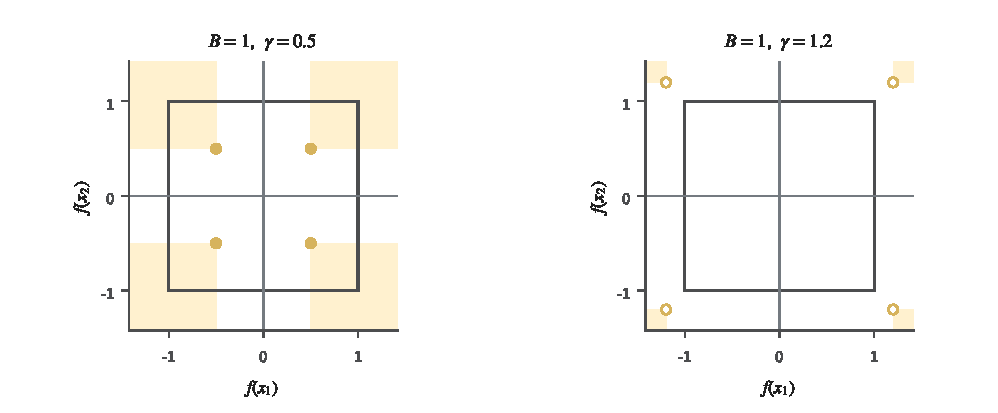
\includegraphics[width=\linewidth]{figures/math-preparation/reader-revision-analysis/combinatorics-fat-margin-output-square.pdf}
 \caption{两个分块、$B=1$与固定阈值$r_1=r_2=0$的输出几何。灰框是函数类允许的
 $(f(x_1),f(x_2))\in[-1,1]^2$；浅黄区域要求两坐标分别离阈值至少$\gamma$。
 左图$\gamma=0.5$的四种符号可由实心点实现；右图$\gamma=1.2$的空心点只标出要求的边界，
 全部落在允许框之外，因而不是类中的函数输出。图为解析教学构造。}
 \label{fig:comb-fat-margin-output-square}
\end{figure*}

组合维度回答函数类能实现哪些模式；一个给定的标记或选择向量是否符合任务约束，
则需要下一节的逻辑规则。

\section{候选空间上的约束与求解}
\label{sec:comb-constrained-solving}

同一个候选空间可以承载不同的任务：规则决定答案是否允许，目标决定允许答案之间怎样
比较，算法保证则说明返回结果的质量。这里回用前章的逻辑语义，明确判定、搜索和优化的
输入输出；随后考察覆盖结构和扩大候选范围分别能给出什么保证。

\subsection{规则系统的判定与搜索任务}
\label{sec:comb-logic-constraints}

第~\ref{chap:sets-functions-and-proofs}章已定义公式的赋值、模型与逻辑后承。
现在把规则作为程序的输入：检查一个给定赋值是否满足、回答有没有满足赋值，以及在有解时
返回一个赋值，是三个不同的任务。前者只检验一个对象，后两者需要处理整个候选空间。

\term{布尔可满足性问题}（Boolean satisfiability problem, SAT）的输入是一个布尔
公式，输出只回答它是否存在满足赋值。输入限制为CNF时称为CNF-SAT；进一步要求每个
子句至多含三个文字时称为\term{3-SAT}。若采用“恰含三个文字”的定义，可以重复文字
补齐较短的非空子句，不改变可满足性；输入若含空子句，则公式立即不可满足。
式~\eqref{eq:comb-running-cnf}因此既是一个CNF-SAT
实例，也是一个3-SAT实例。三者共享“是否存在满足赋值”这一判定接口，但允许的输入
语法不同，不能只凭名称互换实例。

这里回用式~\eqref{eq:comb-running-cnf}的四变量规则。它的模型可以写成
$S(\bm z)=\{i:z_i=1\}$，全部模型恰组成式~\eqref{eq:comb-running-feasible-family}的
五个集合。容斥计算模型数量，SAT只回答是否至少有一个；搜索程序还需实际输出见证。
逻辑后承也可由式~\eqref{eq:comb-entailment-unsat}转为查找反模型，仍须区别语义上的
等价关系与执行这次查找的程序代价。

\subsubsection{逻辑子句与零一约束}

布尔规则也可以写成关于$z_i\in\{0,1\}$的代数约束。一个文字若为$z_i$，
用数值$z_i$表示；若为$\neg z_i$，用$1-z_i$表示。子句
$\ell_1\lor\cdots\lor\ell_r$恰好等价于
\begin{equation}
  \sum_{j=1}^{r}v(\ell_j)\geq1,
  \qquad
  v(z_i)=z_i,\quad v(\neg z_i)=1-z_i.
  \label{eq:comb-clause-linearization}
\end{equation}
因为左侧计算为真的文字个数，至少一个文字为真当且仅当该和不小于$1$。

式~\eqref{eq:comb-running-cnf}因而等价于
\begin{equation}
  z_1+z_2=1,\qquad
  z_3\leq z_1,\qquad
  z_4\leq z_2+z_3,\qquad
  \bm{z}\in\{0,1\}^4.
  \label{eq:comb-running-integer-constraints}
\end{equation}
第一条等式同时包含“至少一个”和“至多一个”。这些条件给出了前章所说的可行域，
其中变量的零一取值条件必须保留。后续第~\ref{chap:optimization}章会进一步研究
可行域的几何结构与求解条件。

若把$\bm{z}\in\{0,1\}^4$放宽为$\bm{z}\in[0,1]^4$，就允许了更多数值候选，
得到一个连续松弛。
分数点
\[
  \bm{z}=(1/2,1/2,1/2,1)
\]
满足全部松弛约束，却不是任何逻辑赋值。按阈值$1/2$把各坐标都取为$1$，还会违反
$z_1+z_2=1$。松弛点可提供优化界或帮助构造整数解，但它本身不是规则系统的合法答案；
取整后必须重新核对原约束。

\subsection{可行选择的目标与近似保证}
\label{sec:comb-optimization-submodularity}

逻辑规则确定哪些集合允许，但通常仍会留下多个答案。
现在给每个可行集合一个数值目标，选择其中最优者；次模性限制增加元素时的边际收益，
从而为贪心近似提供结构保证。计数、可行性和目标值分别属于候选规模、规则与偏好，
不能用其中一项代替另外两项。

\subsubsection{硬规则与偏好代价}

\begin{definition}[硬约束]
\label{def:comb-hard-constraint}
给定候选集合$Z$与必须满足的条件$\phi_1,\ldots,\phi_m$，\term{硬约束}
（hard constraint）把可行集合限定为
$\mathcal C=\{\bm z\in Z:\phi_j(\bm z)\text{为真，对所有}j\}$。
违反任意一条的对象不属于可行集合。
\end{definition}
有些规则表达偏好而非绝对禁止，此时可以为违反规则设置非负代价。令
$r_j(\bm{z})\in\{0,1\}$表示第$j$条规则是否被违反，权重$\lambda_j\geq0$，
则可以最小化
\begin{equation}
  c(\bm{z})+\sum_{j=1}^{m}\lambda_j r_j(\bm{z}),
  \qquad
  \bm{z}\in\{0,1\}^n.
  \label{eq:comb-soft-constraint-objective}
\end{equation}
$c$是任务本身的代价，第二项为规则冲突计分。权重有限时，足够大的任务收益可能抵消
违反规则的代价，所以软规则不再具有逻辑蕴含意义。

把$\lambda_j$取得很大也不能未经证明就等同于硬约束。若$c$的变化范围已知，例如
$|c(\bm{z})-c(\bm{z}')|\leq B$对任意赋值成立，并且存在一个不违反任何软规则的
赋值$\bm{z}_0$，那么令每个$\lambda_j>B$可以排除所有带违反项的全局最优解：
任一违规赋值的目标值严格大于$c(\bm{z}_0)$。若不存在零违反赋值、无法给出可用的
$B$，或希望一族不同规模的实例共用罚权而$c$的振幅没有统一上界，或者只把部分权重
取得较大，这个论证便不成立。
若还为违规程度引入额外变量，同样要说明它们允许哪些原本被排除的赋值。
这些做法各自改变了可行性或比较准则，使用时应明确允许返回什么答案。

\subsubsection{最优解与近似质量}

规则确定集合族$\mathcal{C}\subseteq\mathcal{P}(V)$后，仍需用目标函数比较不同
可行集合。一个有限组合优化问题可写成
\begin{equation}
  \max_{S\in\mathcal{C}}F(S)
  \qquad\text{或}\qquad
  \min_{S\in\mathcal{C}}C(S).
  \label{eq:comb-discrete-optimization}
\end{equation}
由于$\mathcal{C}$有限且非空，实值目标一定达到最优值。这只回答存在性；验证
$S\in\mathcal{C}$、计算$F(S)$以及在不枚举全部候选的情况下找到最优解，仍是不同任务。
存在性的证明只需把$\mathcal{C}=\{S_1,\ldots,S_N\}$列成有限序列：有限个实数
$F(S_1),\ldots,F(S_N)$可逐项比较并取得最大值，达到该值的某个$S_i$就是最优解。
最小化结论可对$-C$应用同一论证。
若$\mathcal{C}=\varnothing$，则没有可行解；若目标允许取无穷值，也需另外说明所用的
大小关系。因此“有限”“非空”和“实值”都是这个存在性结论的条件。

继续使用四个候选。设需求集合为$R=\{a,b,c,d,e\}$，各候选覆盖
\[
  Q_1=\{a,b\},\quad
  Q_2=\{b,c,d\},\quad
  Q_3=\{c,e\},\quad
  Q_4=\{d,e\}.
\]
定义覆盖收益
\begin{equation}
  F(S)=\left|\bigcup_{i\in S}Q_i\right|.
  \label{eq:comb-running-coverage}
\end{equation}
在$\mathcal{C}_0$的五个可行集合上，收益依次为
$2,4,5,3,4$，所以$\{1,3,4\}$达到最优值$5$。这里最优解可以直接列举得到，
因为例子只有五个候选集合；若$n$增大，$2^n$个赋值的枚举时间很快就会成为主要障碍。

只检查局部交换也不能替代全局比较。设可行集合是
$V=\{1,2,3,4\}$的所有二元子集，并规定
$F(\{1,2\})=1$、$F(\{3,4\})=3$，其余二元子集的值均为$0$。
从$\{1,2\}$出发，替换其中任一元素都会使目标降为$0$，所以它是一交换局部最优解；
全局最优解却是$\{3,4\}$。局部最优能否推出全局最优，必须来自目标与可行域的额外结构。

更一般地，对非空集合$X$上的实值目标$f$，记$f^\star=\inf_{x\in X}f(x)$并假设它有限。
给定$\varepsilon>0$，若$\widehat x\in X$且
\begin{equation}
  f(\widehat{x})\leq \inf_{x\in X}f(x)+\varepsilon,
  \label{eq:prelim-epsilon-optimal}
\end{equation}
则称$\widehat{x}$为$\varepsilon$-\term{近似最优解}（approximately optimal
solution）。只要下确界有限，这样的点对每个$\varepsilon>0$都存在；否则
$f^\star+\varepsilon$仍会是一个严格大于下确界的下界，与下确界的定义矛盾。
近似最优描述的是目标值差距，不自动保证$\widehat{x}$接近某个最小点。第~\ref{chap:optimization}章会说明何种曲率条件能把目标误差换成参数距离。

式~\eqref{eq:prelim-epsilon-optimal}要求下确界有限。若目标无下界，只能对每个有限阈值
寻找更低的可行值，不能把$-\infty$当作可达到的最小值，也不能用有限$\varepsilon$表达
到它的距离。

有限最大化问题常另用比例界比较质量。近似解的误差也要先约定口径，而且返回的集合仍须满足原来的规则。
\begin{definition}[乘法近似与加法误差]
\label{def:comb-approximation-guarantee}
设$S^\star$最大化非负目标$F$于非空可行族$\mathcal C$上，算法返回
$\widehat S\in\mathcal C$。若$0\leq\alpha\leq1$且
$F(\widehat S)\geq\alpha F(S^\star)$，称该输出达到$\alpha$乘法近似；
若$\varepsilon\geq0$且$F(S^\star)-F(\widehat S)\leq\varepsilon$，则称其加法误差不超过$\varepsilon$。
\end{definition}
当最优值为$0$或目标可取负值时，乘法比例可能失去区分力，加法误差或经过说明的平移、
归一化口径更合适。

若每个候选还有成本$c_i\geq0$，可以最大化
$F(S)-\sum_{i\in S}c_i$，也可以在预算
$\sum_{i\in S}c_i\leq B$下最大化$F(S)$。这两个问题通常不等价：固定罚权隐含一种
收益与成本交换率，预算约束则禁止所有超额集合。要断言对给定预算存在某个乘子并使
两类问题的最优解对应，还需要额外条件。后续第~\ref{chap:optimization}章会通过
乘子与对偶工具讨论这种对应何时成立；本章的一般离散问题不保证这样的乘子存在，
不能只凭形式相似互换两类问题。

\subsection{覆盖选择的贪心近似}

直接列举最优集合不利用目标结构。覆盖任务中，已经覆盖的需求越多，同一候选能够新增的
需求就越少。这种边际结构可以控制逐步选择损失多少最优收益，但保证还取决于允许的选择规则。

\subsubsection{边际收益与次模性}

一般集合函数可以任意指定每个子集的值，几乎没有可利用的结构。
\begin{definition}[次模函数与边际收益]
\label{def:comb-submodular-function}
\term{次模函数}（submodular function）要求已选择的集合越大，再加入同一元素所得的
边际收益越小。正式地，$F:\mathcal{P}(V)\to\mathbb{R}$若对所有
$A\subseteq B\subseteq V$和$e\in V\setminus B$满足
\begin{equation}
  F(A\cup\{e\})-F(A)
  \geq
  F(B\cup\{e\})-F(B),
  \label{eq:comb-diminishing-returns}
\end{equation}
就称$F$为次模函数。记
\[
  \Delta(e\mid A)=F(A\cup\{e\})-F(A)
\]
后，式~\eqref{eq:comb-diminishing-returns}表示
$\Delta(e\mid A)\geq\Delta(e\mid B)$。
将式~\eqref{eq:comb-diminishing-returns}的不等号反向，即定义超模函数。
\end{definition}

边际随上下文变化的方向，与边际自身是否非负，是两个条件。
\begin{definition}[集合函数的单调性]
\label{def:comb-monotone-set-function}
集合函数$F:\mathcal P(V)\to\mathbb R$具有\term{单调性}（monotonicity），
是指对任意$A\subseteq B\subseteq V$都有$F(A)\leq F(B)$。
等价地，任意允许新增元素的边际收益都非负。
\end{definition}
次模性不等于单调性。次模函数允许边际收益
为负，只要求它随上下文扩大而不增加。模函数
$F(S)=c+\sum_{i\in S}w_i$的边际收益与上下文无关，因此同时是次模和超模函数，
不论某些$w_i$是否为负。

互补收益给出次模性失效的最小反例。令
$G(S)=\mathbb{I}\{\{1,3\}\subseteq S\}$。把元素$3$加入空集的边际收益为$0$，
把它加入$\{1\}$的边际收益却为$1$。由于$0<1$，边际收益随上下文增大而上升，
$G$不是次模函数。这个例子区分了“两个元素共同出现才有收益”的互补关系与覆盖函数中的
替代关系。

次模性还有一个对称的交并形式。

\begin{theorem}[次模性的两个等价定义]
\label{thm:comb-submodular-equivalence}
集合函数$F:\mathcal{P}(V)\to\mathbb{R}$满足边际收益递减
式~\eqref{eq:comb-diminishing-returns}，当且仅当对任意$A,B\subseteq V$有
\begin{equation}
  F(A)+F(B)\geq F(A\cup B)+F(A\cap B).
  \label{eq:comb-submodular-lattice}
\end{equation}
\end{theorem}

\begin{proof}
先假设边际收益递减。把$A\setminus B$中的元素依次记为$e_1,\ldots,e_r$。
从$A\cap B$加入这些元素得到$A$，从$B$加入同一序列得到$A\cup B$。
在第$j$步，前一条路径的当前集合包含于后一条路径的当前集合，因此
\[
  F(A)-F(A\cap B)
  \geq F(A\cup B)-F(B).
\]
移项即得式~\eqref{eq:comb-submodular-lattice}。

反过来，取$A\subseteq B$和$e\notin B$，将交并不等式用于
$A\cup\{e\}$与$B$。二者的交为$A$，并为$B\cup\{e\}$，故
\[
  F(A\cup\{e\})+F(B)
  \geq F(B\cup\{e\})+F(A).
\]
移项便得到式~\eqref{eq:comb-diminishing-returns}。
\end{proof}

\subsubsection{覆盖目标的边际结构}

式~\eqref{eq:comb-running-coverage}是次模性的典型来源。更一般地，为每个需求
$r\in R$给定权重$w_r\geq0$，定义
\begin{equation}
  F(S)
  =
  \sum_{r\in\bigcup_{i\in S}Q_i}w_r.
  \label{eq:comb-weighted-coverage}
\end{equation}

\begin{theorem}[非负加权覆盖函数单调且次模]
\label{thm:comb-coverage-submodular}
若所有$w_r\geq0$，则式~\eqref{eq:comb-weighted-coverage}定义的$F$
是单调次模函数，并满足$F(\varnothing)=0$。
\end{theorem}

\begin{proof}
空集合不覆盖任何需求，所以$F(\varnothing)=0$。若$A\subseteq B$，则$A$覆盖的
需求也被$B$覆盖；权重非负保证$F(A)\leq F(B)$。对
$A\subseteq B$和$e\notin B$，加入$e$的边际收益是
\[
  \Delta(e\mid A)
  =
  \sum_{r\in Q_e\setminus\bigcup_{i\in A}Q_i}w_r.
\]
由于
$\bigcup_{i\in A}Q_i\subseteq\bigcup_{i\in B}Q_i$，在$B$的基础上尚未覆盖的
$Q_e$元素不会比在$A$的基础上更多。逐项使用$w_r\geq0$，得到
$\Delta(e\mid A)\geq\Delta(e\mid B)$。
\end{proof}

在贯穿例子中，候选$3$单独加入空集时新增$\{c,e\}$，边际收益为$2$；若已经选择
$\{2\}$，需求$c$已经覆盖，加入$3$只新增$e$，边际收益降为$1$。这个计算展示了
式~\eqref{eq:comb-diminishing-returns}的一种情形，但一般结论来自上面的集合包含
证明，而不是来自一个数值例子。

非负权重是单调性证明的实质条件。若某个被覆盖对象具有负权重，增加候选可能降低目标；
函数是否仍次模要按具体形式检查。两个次模函数之和仍次模，非负倍数也保持次模性，
但次模函数之差一般不次模。给覆盖收益减去模块化成本仍是次模函数，却可能失去单调性。

图~\ref{fig:combinatorics-coverage-marginals}在同一个新增候选上核对边际递减：候选\(3\)覆盖\(\{c,e\}\)，背景为空时新增两个需求；背景为\(\{2\}\)时只新增\(e\)；背景进一步扩大为\(\{2,4\}\)时不再新增需求。这三个嵌套背景允许比较同一个元素的边际，而对不相包含的背景任意排出柱高次序，并不能验证次模性。

\begin{figure}[htbp]
  \centering
  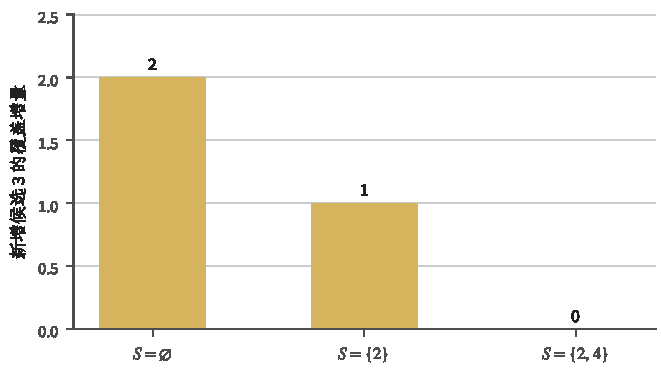
\includegraphics[width=\linewidth]{figures/math-preparation/probability-discrete/combinatorics-coverage-marginals.pdf}
  \caption{覆盖函数的有限教学构造。使用式~\eqref{eq:comb-running-coverage}中的\(Q_2,Q_3,Q_4\)，向\(\varnothing\subset\{2\}\subset\{2,4\}\)分别加入候选\(3\)，覆盖增量为\(2,1,0\)。柱高从零基线起画；图中只展示一个具体递减链，完整次模性仍由集合差证明。}
  \label{fig:combinatorics-coverage-marginals}
\end{figure}

\subsubsection{基数约束下的贪心保证}

次模性约束边际收益之间的关系，但只有与特定可行域和算法结合，才能得到求解保证
\scite{math-nemhauser1978submodular}
考虑归一化单调次模最大化
\[
  \max_{S\subseteq V,\ |S|\leq k}F(S),
  \qquad F(\varnothing)=0.
\]
贪心算法从$S^{(0)}=\varnothing$开始，在第$t$步选择边际收益最大的元素
\[
  e^{(t)}\in\argmax_{e\in V\setminus S^{(t)}}\Delta(e\mid S^{(t)}),
  \qquad
  S^{(t+1)}=S^{(t)}\cup\{e^{(t)}\}.
\]
平局可按固定顺序处理，使算法输出确定。

\begin{theorem}[单调次模最大化的贪心界]
\label{thm:comb-greedy-submodular}
设$1\leq k\leq|V|$，$F$归一化、单调且次模，$S^\star$是在
$|S|\leq k$下的最优解。
上述贪心算法运行$k$步得到$S^{(k)}$，则
\begin{equation}
  F(S^{(k)})
  \geq
  \left(1-\left(1-\frac1k\right)^k\right)F(S^\star)
  \geq(1-e^{-1})F(S^\star).
  \label{eq:comb-greedy-bound}
\end{equation}
\end{theorem}

\begin{proof}
固定第$t$步。由单调性、次模性以及逐个加入$S^\star\setminus S^{(t)}$中的元素，
\begin{align*}
  F(S^\star)-F(S^{(t)})
  &\leq F(S^{(t)}\cup S^\star)-F(S^{(t)})\\
  &\leq\sum_{e\in S^\star\setminus S^{(t)}}\Delta(e\mid S^{(t)}).
\end{align*}
右侧至多有$k$项，所以其中至少一项不小于
$[F(S^\star)-F(S^{(t)})]/k$。若右侧没有元素，则单调性已经给出
$F(S^{(t)})\geq F(S^\star)$，所需递推平凡成立；否则贪心选择的边际收益不小于上述某一项，
故
\[
  F(S^{(t+1)})-F(S^{(t)})
  \geq\frac{F(S^\star)-F(S^{(t)})}{k}.
\]
令剩余差距$r^{(t)}=F(S^\star)-F(S^{(t)})$，便有
$r^{(t+1)}\leq(1-1/k)r^{(t)}$。由$F(S^{(0)})=0$递推得到
\[
  r^{(k)}\leq\left(1-\frac1k\right)^kF(S^\star),
\]
移项给出第一个不等式。再用初等指数不等式$1-u\leq e^{-u}$（$0\leq u\leq1$），
得到$(1-1/k)^k\leq e^{-1}$，从而得到第二个不等式。
\end{proof}

定理~\ref{thm:comb-greedy-submodular}不能直接套到
式~\eqref{eq:comb-running-feasible-family}。逻辑规则形成的$\mathcal{C}_0$
不是普通基数约束，甚至不是向下封闭的：$\{1,3\}$可行，其子集$\{3\}$却不可行。
逐个加入当前边际收益最大的元素可能在中途违反规则，或走入无法扩展到最优解的分支。
其他约束下可以有不同的贪心、连续松弛或近似结果，但保证必须重新证明，不能只凭目标
具有次模性。

\subsection{扩大候选范围的最优值界}

把每个可行集合$S\in\mathcal C$写成指示向量$\bm z(S)\in\{0,1\}^n$，
得到整数可行点集$Z$。若用$P\subseteq[0,1]^n$放宽候选范围，就要求$Z\subseteq P$。
在$P$上选定目标$G$，并让$G(\bm z(S))=F(S)$对全部原候选成立，则
\[
  \max_{S\in\mathcal C}F(S)\leq\sup_{\bm z\in P}G(\bm z).
\]
原因只是原候选仍在扩大后的范围内；这里假设$\mathcal C$有限、非空且$F$实值。
任何取整后仍满足原规则的解则给出最大化目标的下界。对最小化问题，上下界方向相反。

例如考虑
\[
  \max\ z_1+z_2
  \quad\text{s.t.}\quad
  2z_1+2z_2\leq3,\qquad z_1,z_2\in\{0,1\}.
\]
整数最优值为$1$。放宽为$0\leq z_1,z_2\leq1$后，约束给出
$z_1+z_2\leq3/2$，而$(z_1,z_2)=(1,1/2)$恰好达到$3/2$，所以它是松弛最优值，
确实是整数最优值的上界。
若把正坐标都取为$1$，则得到$(1,1)$并违反容量约束；若把$1/2$向下取整，则恢复一个
值为$1$的可行解。这个算例同时展示了松弛界、取整可行性与取整后目标值是三项不同检查。

本小节只利用候选范围的包含关系建立界。松弛集合的几何结构如何影响最优值，
以及取整后的可行性与目标误差怎样判断，将在后续第~\ref{sec:opt-relaxations-certificates}节
展开；目标具有次模性本身还不足以回答这些问题。

\section{问题族的可计算性与复杂度}
\label{sec:comb-computability-complexity}

前节规定了什么结果算作合法答案，并给出了特定选择算法的质量保证。
现在把考察对象换成整类输入及处理它们的统一程序：程序是否对规定输入正确终止，以及
时间、空间和证书规模怎样随输入增长，是两类独立要求。
通用可计算性并不从属于候选计数；即使每个实例都由有限字符串编码，关于程序行为的
整个问题族仍可能不可判定。有限候选可枚举与枚举成本可承受也须分开。

\subsection{输入编码与计算模型}

复杂度不是对象本身附带的标签，而是相对于输入编码、计算模型和所求输出定义的。
对有限变量问题，可以把$n$、CNF公式、整数或有理数权重以及阈值写成有限比特串。
输入长度记为$L$，它包括变量索引、子句、数值的二进制位数和分隔信息。
若一个权重需要$b$位表示，读取和比较它就不能无条件算作与$b$无关的一步。

同一优化任务常对应三个不同计算问题。
\begin{itemize}
  \item \term{搜索问题}要求返回一个满足$\Phi$的$\bm{z}$；
  \item \term{优化问题}要求返回目标最优的可行$\bm{z}$或最优值；
  \item \term{判定问题}只问是否存在满足$\Phi$且$F(S(\bm{z}))\geq K$的赋值。
\end{itemize}
复杂性类别通常先为判定问题定义。若能多次调用判定算法并固定变量，常可恢复一个解；
但调用次数、数值精度和自归约结构都要计入，不能把“知道答案存在”直接当作已经构造答案。

\subsection{可枚举、可判定与可计算}

按顺序输出候选、回答某个输入是否属于集合，以及计算一个函数值，要求程序提供不同的
信息。特别是等待某个候选出现时，暂时没有看到它，并不能给出“永远不会出现”的答案。
下面都以有限字符串作为输入编码，以一个固定、有限描述的程序处理全部允许输入。
\begin{definition}[可枚举、可判定与可计算]
\label{def:comb-computability}
一个对象集合若存在程序依次输出其中全部对象，称为\term{可枚举的}
（computably enumerable）。这里要求程序只输出该集合中的对象，并最终输出其中每个
对象；程序可以重复输出，也不必告诉我们某个尚未出现的对象
以后是否会出现。一个判定问题若存在程序对每个合法输入都在有限步内停机，并正确回答
“是”或“否”，称为\term{可判定的}（decidable）。若程序只保证在“是”实例上最终
停机并接受，而在“否”实例上可能永不停止，则称该问题\term{半可判定的}
（semidecidable）。
类似地，定义在全部有限字符串上的函数$f$若存在一个程序，对每个输入$x$都停机并输出
$f(x)$，就称$f$为\term{可计算函数}（computable function）。若讨论部分函数，
还要求程序恰在其定义域内停机并输出相应值，域外输入不停止；仅承诺处理一个指定子集
属于另一种带输入承诺的问题约定。
\end{definition}
判定问题可看作计算
取值为$0$或$1$的特征函数，因此可判定性比只确认正例的半可判定性要求更强。

可枚举不等于可判定。若某集合及其补集都可枚举，可以交错运行两个枚举或半判定程序：
输入最终会被其中一方确认，于是得到判定程序。若只有正例可枚举，等待尚未出现的对象
无法证明它永远不会出现。

在明确的有限编码下，CNF可满足性是可判定的。按字典序枚举全部
$2^n$个赋值，每个赋值逐子句检查；找到满足赋值就回答“是”，全部检查完仍未找到则
回答“否”。若公式有$m$个子句、总文字出现次数为$q$，直接实现需要
$O(2^n q)$量级的时间和存放当前赋值及公式所需的空间。这个算法很慢，但一定停机，
所以它证明了可判定性。

“每个实例的候选集有限”还不足以独立构成上述证明。程序必须能从输入有效得到候选编码，
能判定一个候选是否满足约束，并能知道枚举何时完成。若把一个不可计算实数或一个可能
不停机的黑盒藏进“目标求值”，有限个候选也未必能被统一程序比较。可计算性要求的是
对整族输入存在同一个有限描述的程序。

\subsection{不可判定性与停机问题}

有限变量问题在有效表示下可以穷举，但一般程序的行为并非总能判定。
令
\[
  \mathrm{HALT}
  =
  \{(P,x):\text{程序 }P\text{ 在输入 }x\text{ 上最终停机}\}.
\]
它是半可判定的：模拟$P(x)$，若模拟停止就接受；若$P(x)$永不停止，模拟也不会给出
否定答案。下面的对角论证说明不存在总能判断停机与否的程序。

停机问题的不可判定性是可计算性理论的基本结论\scite{math-turing1937computable}
\begin{theorem}[停机问题不可判定]
\label{thm:comb-halting-undecidable}
$\mathrm{HALT}$不可判定。
\end{theorem}

\begin{proof}
反设存在判定程序$H(P,x)$，它总会停机，并在$P(x)$停机时返回$1$，否则返回$0$。
据此构造程序$D$：输入一个程序编码$P$，先计算$H(P,P)$；若结果为$1$，就进入无限
循环；若结果为$0$，就立即停机。

现在把$D$自己的编码交给$D$。若$H(D,D)=1$，按照$D$的定义，$D(D)$进入无限循环，
与$H$判断它会停机矛盾。若$H(D,D)=0$，$D(D)$立即停机，又与$H$判断它不停机矛盾。
两种返回值都导致矛盾，所以这样的判定程序$H$不存在。
\end{proof}

定理~\ref{thm:comb-halting-undecidable}区分了“某次模拟尚未结束”和“已经证明不会结束”。
前者是有限时刻的观察，后者要求排除所有未来时刻。不可判定也不等于每个具体程序都无法
分析；许多程序可由终止度量、循环不变量或有限状态搜索证明停机。结论是不存在一个对
任意程序和输入都正确的统一判定器。

\subsection{多项式时间、证书与复杂性类别}

可判定问题仍可能需要随输入长度急剧增长的资源。能统一快速求解，与只能快速核对给定答案，
是不同的计算要求。
\begin{definition}[复杂性类别P与NP]
\label{def:comb-p-np}
若存在一个对所有实例都正确判定的确定性算法，其最坏运行时间由
$L$的某个固定次数多项式控制，该判定问题属于复杂性类别$\mathrm{P}$。
类别$\mathrm{NP}$包含满足如下条件的判定问题$\mathcal{L}$：存在多项式$p$和确定性
多项式时间验证程序$\mathsf{Ver}$，使每个输入$x$都满足
\[
  x\in\mathcal{L}
  \quad\Longleftrightarrow\quad
  \exists y,\quad |y|\leq p(|x|),\quad \mathsf{Ver}(x,y)=1.
\]
其中$|x|$是输入的比特长度，$y$称为\term{证书}（certificate）。
\end{definition}
双向条件不仅要求
每个“是”实例存在可接受的多项式长度证书，还要求“否”实例的所有这类证书都被拒绝。
名称中的“非确定性”描述这种猜测证书后验证的计算模型，不表示算法可以容忍随机错误。
确定性多项式算法的运行轨迹本身可作证书，所以
$\mathrm{P}\subseteq\mathrm{NP}$。目前并不知道这个包含是否严格；把
$\mathrm{P}\neq\mathrm{NP}$当作已经证明的事实，会超出这里可用的结论。

CNF可满足性属于$\mathrm{NP}$。证书就是$n$位赋值$\bm{z}$，验证程序逐个检查子句，
时间关于公式长度为线性量级。穷举证明它可判定，短证书证明它属于$\mathrm{NP}$；
二者都没有给出多项式时间的求解算法。

\begin{definition}[多项式时间多对一归约]
\label{def:comb-polynomial-reduction}
若判定问题$A$的每个实例$x$都能在多项式时间内变换为判定问题$B$的实例$f(x)$，并满足
\[
  x\in A\quad\Longleftrightarrow\quad f(x)\in B,
\]
就称$A$可\term{多项式时间多对一归约}（polynomial-time many-one reduction）
到$B$，记作$A\leq_{\mathrm{p}}B$。
\end{definition}
归约方向表示：若能高效解决$B$，就能先计算
$f(x)$再高效解决$A$。因此从已知困难问题归约到新问题，才能证明新问题至少同样困难；
把方向写反不会得到这个结论。

\begin{definition}[NP困难与NP完全]
\label{def:comb-np-hard-complete}
一个判定问题若所有$\mathrm{NP}$问题都可多项式时间归约到它，就称为
\term{NP困难}（NP-hard）；若它还属于$\mathrm{NP}$，就称为
\term{NP完全}（NP-complete）。
\end{definition}
Cook--Levin定理给出SAT是NP完全问题
\scite{math-cook1971complexity}通过引入
辅助变量，可以把一般公式在多项式时间内变成等可满足的CNF公式；再把长子句拆成由辅助
变量连接的三文字子句，可以归约到3-SAT。这里的“等可满足”只保证原公式有解当且仅当
新公式有解，不要求辅助变量加入后两个公式拥有相同的模型集合。由这些接口可知CNF-SAT
与3-SAT也都是NP完全问题。这里把结论作为复杂度理论的基准，不展开对任意多项式时间
验证计算的编码证明；下面只证明与本章约束表示直接相关的归约。

\begin{theorem}[CNF可满足性归约到零一线性可行性]
\label{thm:comb-sat-to-binary-linear}
给定任意CNF公式，可以在关于公式长度的多项式时间内构造一组零一线性不等式，
使该公式可满足当且仅当这些不等式存在零一可行解。因此零一线性可行性是NP困难的；
当所有整数系数按二进制编码时，它也属于NP，因而是NP完全的。
\end{theorem}

\begin{proof}
为每个命题变量建立$z_i\in\{0,1\}$。对每个子句
$C=\ell_1\lor\cdots\lor\ell_r$，加入式~\eqref{eq:comb-clause-linearization}：
\[
  \sum_{j=1}^{r}v(\ell_j)\geq1.
\]
每个文字只产生一个系数为$1$的变量项或$1-z_i$，所以构造时间和输出长度都关于原公式
长度为线性量级。

若原公式有满足赋值，把真假分别编码为$1,0$。每个子句至少一个文字为真，对应不等式
左侧至少为$1$，所以得到零一可行解。反过来，任一零一可行解定义一个布尔赋值；
每条不等式左侧至少为$1$，说明相应子句至少一个文字为真，故全部子句同时满足。
两边可行性等价，归约成立。

由CNF可满足性的NP困难性，零一线性可行性NP困难。对其NP成员关系，证书是一组零一
变量值；验证者按二进制整数运算检查所有不等式，所需时间关于输入和证书长度为多项式。
\end{proof}

定理~\ref{thm:comb-sat-to-binary-linear}说明，换成代数记号不会自动消除逻辑搜索的
困难。它也没有声称每个零一线性实例都难：式~\eqref{eq:comb-running-integer-constraints}
只有四个变量，可以立即求解；某些约束矩阵或关系结构还允许专门的多项式算法。
NP完全描述的是一族问题在最坏情况下的归约地位，不是每个实例的运行时间预测。

\subsection{复杂度结论的边界}

输入规模必须与算法成本使用同一口径。枚举$2^n$个赋值是关于变量数$n$的指数时间；
若输入本身已经显式列出全部$2^n$个候选，那么扫描列表反而关于输入长度是线性的。
把隐式表示与显式列表混在一起，会让同一算法同时被误称为指数和线性。

数值大小也不能替代编码长度。若整数$N$用二进制给出，输入它只需
$\lfloor\log_2N\rfloor+1$位；执行$N$轮的循环关于数值$N$是线性的，却关于输入位数
是指数级的。运行时间关于数值大小是多项式、关于二进制输入长度却未必是多项式的算法，
称为\term{伪多项式时间算法}（pseudo-polynomial-time algorithm）。只有同时说明
数值编码与所计基本运算，才能判断一个界是否真正关于输入长度为多项式。

最坏情况复杂度也不同于一次实验运行时间。某个求解器在当前数据上很快，可能来自实例
结构、预处理或启发式分支顺序；这不能证明问题属于$\mathrm{P}$。反过来，NP完全性
不排除小实例、特殊结构、参数受限情形或近似目标能够高效求解。应说明保证针对精确解、
近似值还是可行解，并列明依赖的参数与表示。

统计样本量与计算时间同样不能互相替代。一个候选族可能只需较少样本就能控制泛化误差，
经验风险最小化却仍难以计算；也可能存在高效优化算法，但样本不足以区分多个预测规则。
可计算学习还要求训练程序和输出的预测程序都停机，高效学习进一步要求相应资源由规定
参数的多项式控制。组合计数可以进入统计界，也可以进入枚举成本，但两处的规模对象和
结论必须分别核对。

\subsection{数学答案与程序保证的区别}

程序保证需要与数学答案的性质分开。回看式~\eqref{eq:prelim-regularized-least-squares}，
“求一个最小值”至少涉及下面四种不同要求，计算资源还在可计算性之外另加限制。

\begin{table}[htbp]
  \centering
  \small
  \begin{tabularx}{\linewidth}{@{}lX@{}}
    \toprule
    \textbf{问题} & \textbf{需要回答的内容} \\
    \midrule
    存在性 & 是否有$\bm{w}^\star$真正达到$\inf_{\bm{w}}F(\bm{w})$。 \\
    唯一性 & 达到最优值的参数是否只有一个。 \\
    可识别性 & 不同参数是否会产生相同的可观测预测或数据分布。 \\
    可计算性 & 是否有对规定输入终止并给出正确结果的统一程序；精度和资源界需另行说明。 \\
    \bottomrule
  \end{tabularx}
  \caption{最优化陈述中的四类不同要求。每一行需要不同的条件与论证。}
  \label{tab:prelim-four-solution-questions}
\end{table}

这四类问题彼此相关，却不能相互替代。一个有限非空候选集上的实值函数必定达到最小值，
但若没有给出枚举候选或计算函数值的有效方式，存在性本身不提供实际算法。例
\ref{ex:prelim-nonidentifiable-parameterization}中的参数不可唯一识别，但乘积$ab$
对应的预测函数仍可唯一确定。反过来，即使目标函数只有一个最小点，有限精度计算通常也
只能返回近似值；能否精确到达该点，或能在多大误差内逼近它，需要单独的算法保证。

回到带正则项的最小二乘。它的变量属于$\mathbb{R}^d$，目标值属于$\mathbb{R}$，
样本索引$i$遍历同一组$n$个观测，$\lambda$控制第二项的权重。若要声称某算法返回唯一
的目标最优点，需要分别证明最小点存在、最小点唯一，以及算法确实到达该点；若算法只给出
误差保证，则应改称它在规定成本下得到近似解。只有进一步声称该参数可由观测唯一确定，
或算法恢复了真实参数时，才需要额外证明数据与参数化具有所需的可识别性。后续章节将在
各自需要时分别给出这些条件。

\section{本章小结}
\label{sec:comb-summary}

候选空间、求解任务和程序是三个不同的考察对象。精确计数与增长尺度说明结果数量怎样
变化，容斥校正重叠，Möbius反演恢复累计量中的局部贡献。函数族的限制类记录有限输入上
可实现的标记；VC维及多类别维度约束模式丰富度，实值函数还要固定阈值与间隔。
这些容量结论不直接给出训练或求解算法的运行时间。

规则与目标共同规定答案。检查一个赋值、判定有解、构造见证与取得最优结果不能混用；
子句的零一转换保持逻辑可行性，连续松弛和软代价则改变允许对象或比较准则。
覆盖的边际递减配合单调性与基数约束，才能给出贪心质量界；松弛界还需另外检查取整后的
可行性和目标误差。存在一个最佳候选，并不自动给出找到它的程序。

统一程序必须处理规定的整类输入。可枚举、可判定与可计算分别说明程序能提供什么回答，
停机问题展示一般程序任务的不可判定边界；多项式时间、证书与归约则讨论资源和困难度。
结果数量、答案质量、终止保证、计算成本与统计样本量各有自己的对象和条件。
当候选连续变化或迭代无限延续时，还需第~\ref{chap:mathematical-analysis}章的
测度、极限与连续性工具；第~\ref{chap:graph-theory}章会进一步研究关系结构怎样改变
路径、分离和计算组织。
